The \dword{ce} signal processing is implemented in application-specific integrated circuits (\dwords{asic})
using \dword{cmos} technology.  The \dword{ce} is continuously read out, resulting in a digitized \dword{adc}
sample from each \dword{apa} channel (wire) up to every \SI{500}{ns} (\SI{2}{MHz} sampling rate).

Each individual \dword{apa} has \num{2560} channels that are read out by \num{20} %front-end motherboards (
\dfirsts{femb}, with
each \dshort{femb} enabling digitized wire readout from \num{128} channels.  One cable bundle connects each \dword{femb} to
the outside of the cryostat via a \dword{ce} signal cable flange located at the \dword{ce} \fdth at the
top of the cryostat, where a single flange services each \dword{apa}, as shown in Figure~\ref{fig:connections}.  Two \dword{ce} signal flanges are located on each \fdth, together accounting for all electronics channels associated with a pair of \dwords{apa} (upper and lower, vertically arranged).
Each cable bundle contains wires for low-voltage (\dword{lv}) power, high-speed data readout, and
clock or digital-control signal distribution.  Eight separate cables carry the TPC wire bias voltages
from the signal flange to the \dword{apa} wire bias boards, in addition to the bias voltages for the field
cage termination electrodes and for the electron diverters.  An addition flange on the top of each \fdth services the \dword{pds} cables associated with the \dword{apa} pair.

\begin{dunefigure}
[Connections between the signal flanges and \dword{apa}]
{fig:connections}
{Connections between the signal flanges and \dword{apa}. Only the upper \dword{apa} of the hanging \dword{apa} pair, described in Section~\ref{sec:fdsp-apa-frames}, and its connection paths are shown. The lower \dword{apa} will share the \dword{pd} flange with the upper \dword{apa} but have a separate TPC readout flange. A \textit{\dword{ce} module} consists of all \dword{ce} associated with \num{128} channels of digitized readout.}
%\hspace{1cm}
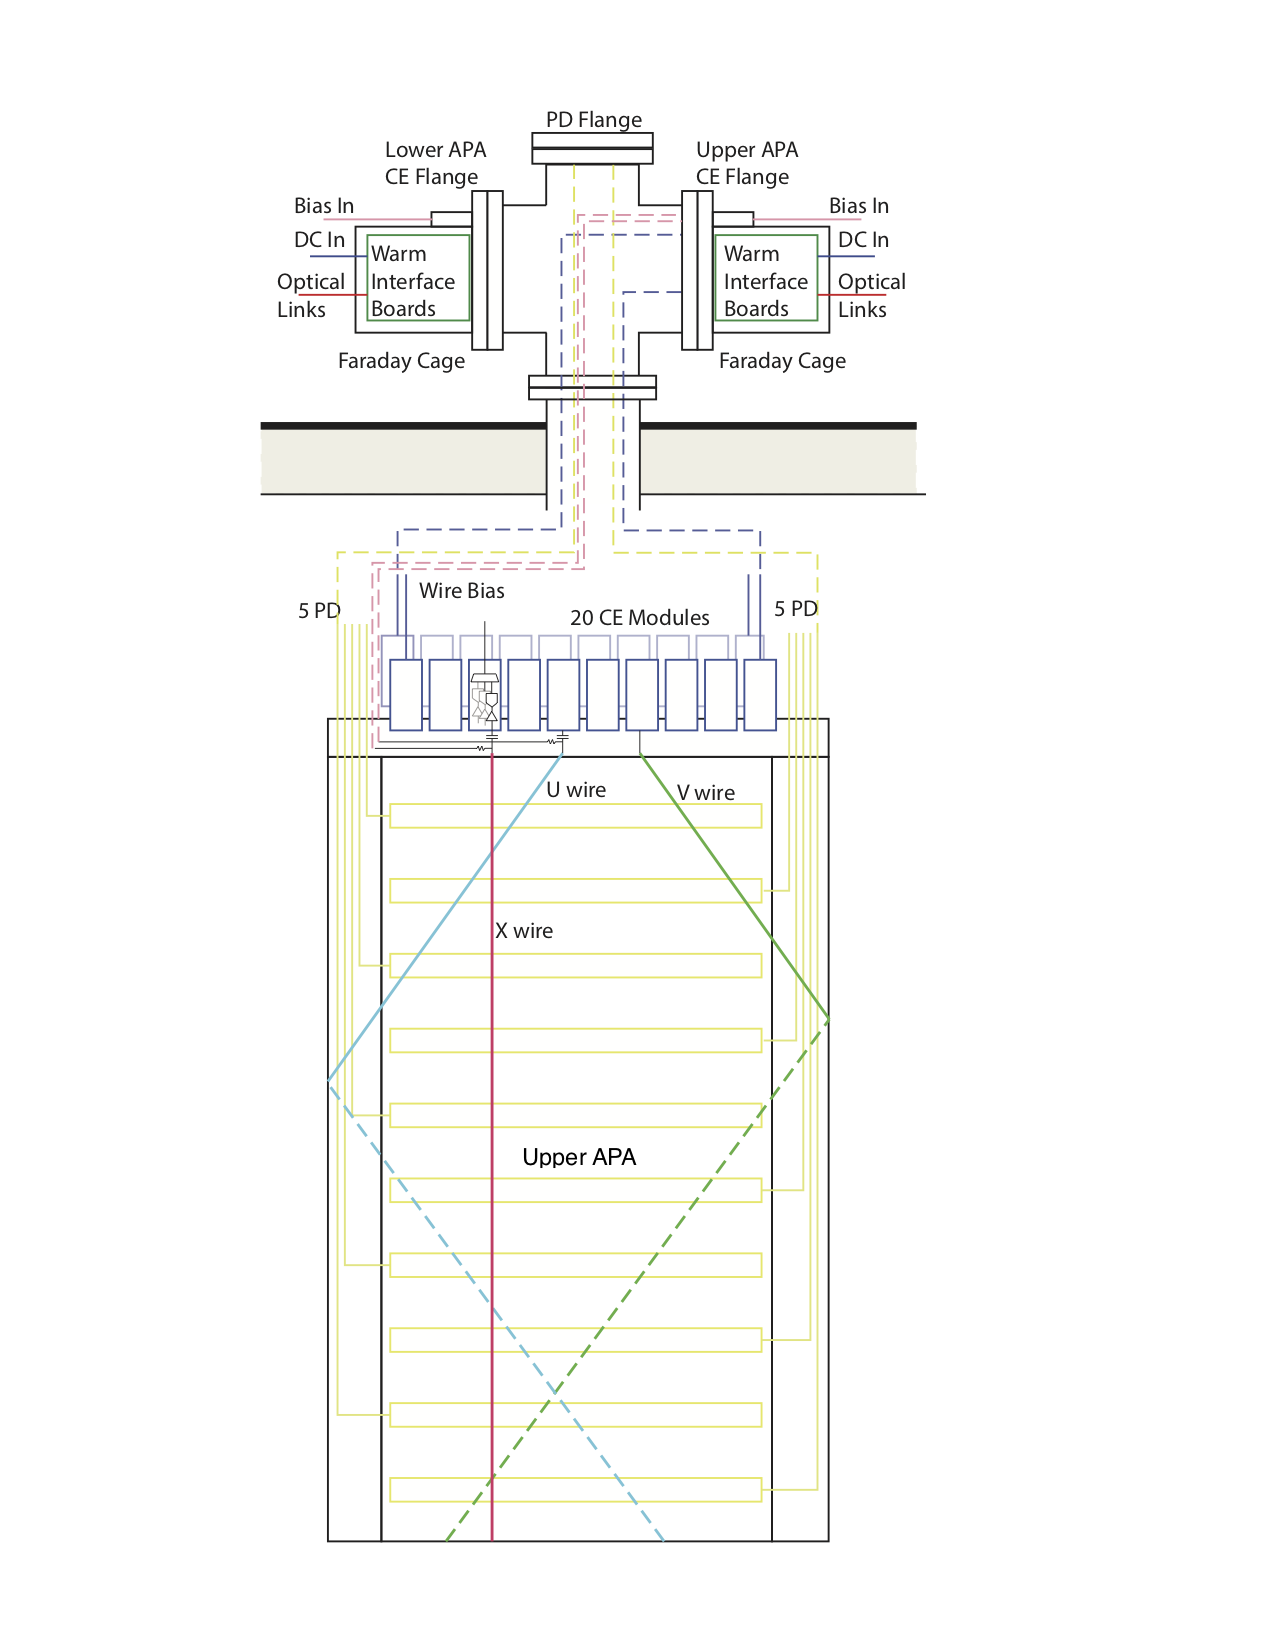
\includegraphics[width=0.9\textwidth]{tpcelec-PDSP_Connections.png}
\end{dunefigure}

The components of the \dword{ce} system are the following:
\begin{itemize}
\item{\dwords{femb}, on which the \dwords{asic} are mounted, which are installed on the \dwords{apa};}
\item{cables for the data, clock and control signals, \dword{lv} power, and wire bias voltages between the \dword{apa} and the signal flanges (cold cables);}
\item{signal flanges with a \dword{ce} \fdth to pass the data, clock and control signals, \dword{lv} power, and \dword{apa} wire-bias voltages between the inside and outside of the cryostat, in addition to the corresponding cryostat penetrations and spool pieces;}
\item{%warm interface electronics crates (
\dwords{wiec} that are mounted on the signal flanges and contain
the %warm interface boards (
\dwords{wib} and %power and timing cards (
\dwords{ptc} for further processing
and distribution of the signals entering and exiting the cryostat;}
%\item{fiber cables for transmitting data and clock/control signals between the \dwords{wiec} and the
%data acquisition (DAQ) and slow control systems;}
\item{cables for \dword{lv} power and wire bias voltages between the signal flange and external power
supplies (warm cables); and}
\item{\dword{lv} power supplies for the \dword{ce} and bias-voltage power supplies for the \dwords{apa}.}
\end{itemize}

Table~\ref{tab:elecNums} lists the component type, the quantity required for each type  and the number of channels per component of each type.

\begin{dunetable}
[TPC electronics components and quantities for a single \dword{apa} of a %the DUNE \single 
\dword{spmod}.]
{llr}
{tab:elecNums}
{TPC electronics components and quantities for a single \dword{apa} of the DUNE \dword{spmod}.}
\textbf{Element} &\textbf{Quantity} & \textbf{Channels per element}\\ \toprowrule
Front-end mother board (\dword{femb}) & \num{20} per \dword{apa} & \num{128} \\ \colhline
FE \dword{asic} chip & \num{8} per \dword{femb} & \num{16} \\ \colhline
\dword{adc} \dword{asic} chip & \num{8} per \dword{femb} & \num{16} \\ \colhline
\dword{coldata} \dword{asic} chip & \num{2} per \dword{femb} & \num{64} \\ \colhline
Cold cable bundle & \num{1} per \dword{femb} & \num{128} \\ \colhline
Signal flange & \num{1} per \dword{apa} & \num{2560} \\ \colhline
\dword{ce} \fdth & \num{1} per \dword{apa} & \num{2560} \\ \colhline
Warm interface board (\dword{wib}) & \num{5} per \dword{apa} & \num{512} \\ \colhline
Warm interface electronics crate (\dword{wiec}) & \num{1} per \dword{apa} & \num{2560} \\ \colhline
Power and timing card (\dword{ptc}) & \num{1} per \dword{apa} & \num{2560} \\ \colhline
Power and timing backplane (PTB) & \num{1} per \dword{apa} & \num{2560} \\
%\dword{lv} power mainframe & ? & ? \\ \colhline
%\dword{lv} supply module & ? & ? \\ \colhline
%wire bias mini-crate & ? & ? \\ \colhline
%wire bias supply module & ? & ? \\
\end{dunetable}

The baseline design for the \dword{spmod} TPC electronics calls for three types of \dwords{asic} to be located inside of the \lar:
\begin{itemize}
\item{a \num{16}-channel \dword{fe} \dword{asic} for amplification and pulse shaping, referred to as \dword{larasic} in the following;}
\item{a \num{16}-channel \num{12}-bit \dword{adc} \dword{asic} operating at \SI{2}{MHz}; and}
\item{a \num{64}-channel control and communications \dword{asic}, referred to as \dword{coldata} in the following.}
\end{itemize}

The \dword{fe} \dword{asic} has been prototyped and is close to meeting requirements (discussed in Section~\ref{sec:fdsp-tpc-elec-ov-req}). Another prototype to address issues in the version deployed in \dword{pdsp} is expected in the spring of 2018. Key portions of the control and communications \dword{asic} (also referred to as the \dword{coldata} \dword{asic}) have been prototyped and meet requirements.  However, it has been determined that the BNL-designed P1-\dword{adc} \dword{asic} now being used in \dword{pdsp} does not meet requirements, and accordingly, its development has been terminated.  A new \dword{adc} \dword{asic} (referred to as the cold \dword{adc} \dword{asic}) is being developed by an LBNL-\fnal-BNL collaboration and first prototypes are expected by the end of summer 2018.  The first full prototype of the controls and communication \dword{asic} is also expected to be available for testing by the end of summer 2018. 

In order to maximize the probability of developing a complete design for cold TPC \dword{fe} electronics in a timely fashion, an alternative solution is also being investigated, a single \num{64}-channel \dword{asic} that will consolidate all three functions described above.  This design is being done at SLAC and first prototypes are expected in summer 2018.  An \dword{adc} solution in the form of a developmental \dword{adc} chip for an upgrade of the ATLAS detector provides an additional backup option; this option will be explored further if the performance of the other two \dword{adc} solutions being considered do not meet the requirements for DUNE.

While the higher charge carrier mobility at \lar temperature than at room temperature is central to the improved performance of \dword{ce}, it also leads to the \textit{hot carrier effect}.  In n-type MOS transistors, the carriers (electrons) can acquire enough kinetic energy to ionize silicon in the active channel.  This charge can become trapped and lead to effects (including threshold shifts) similar to those caused by radiation damage.  This effect can cause MOS circuits to age much more quickly at \lar temperature than at room temperature, reducing performance and potentially causing failure.  In order to mitigate this effect, the maximum \efield in transistor channels must be lower than the field that can be reliably used at room temperature.  
This is accomplished by using transistors that are fabricated with longer than typical length and operated at reduced bias voltage.  Any commercial circuits that are used in the \lar must be carefully tested to ensure that they will perform well for the expected \num{20}-year lifetime of DUNE.

A series of tests are planned to demonstrate that the \dword{ce} system design will meet DUNE requirements. These include two system tests: one using the \dword{pdsp} \textit{cold box} at CERN, and one using a new small \lartpc at \fnal. The latter will also accommodate one half-length DUNE \dword{pd}, and will provide a low-noise environment that will allow one to make detailed comparisons of the performance of the new \dwords{asic}. It will also enable the study of interactions between the TPC readout and other systems, including the \dword{pd} readout and the \dword{hv} distribution. These test facilities are discussed in more detail in Section~\ref{sec:fdsp-tpc-elec-qa-facilities}. Plans are also being made for a second period of data taking for the \dword{pdsp} detector, with final \dwords{apa} including the final \dwords{asic} and \dwords{femb} replacing the current prototypes. This second run of \dword{pdsp} is planned for 2021-2022.
